\section{BIOS}

% - motivace
% - pouziti cc65 a neslib
% - jako priklad NES programu
% - ukazka struktury a pouziti neslib
% - ukazka komunikace FWX

BIOS představuje první software, který emulovaný CPU po spuštění vykoná. V tomto projektu neplní
BIOS pouze funkci inicializace hardwaru, ale slouží jako grafické uživatelské rozhraní pro výběr
programů z SD karty.

Hlavní motivaci pro tvorbu vlastního BIOSu bylo poskytnout uživateli jednoduchý a přivětivý způsob k
výběru programu pro načtení a konfiguraci zařízení. Řešením by bylo vytvořit interaktivní menu, kde
uživatel bude moci procházet souborový systém SD karty nebo přejít do režimu nastavení.

\begin{figure}[H]
    \centering
    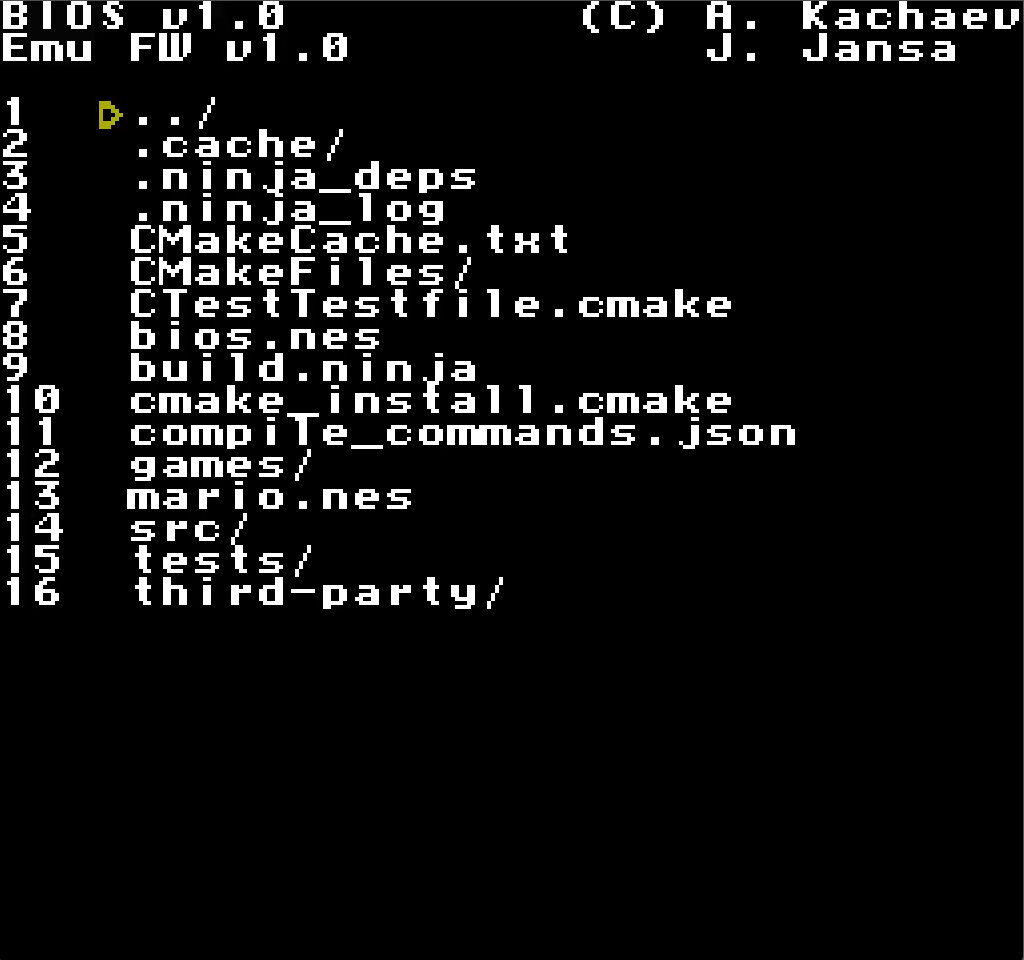
\includegraphics[width=0.55\textwidth]{images/bios.png}
    \caption{Ukázka hlavního menu BIOS.}
    \label{fig:bios}
\end{figure}

Pro realizaci BIOSu byl použit kompilátor cc65, který umožňuje psát kód v jazyce C. Použití
assembleru 6502 pro komplexnější logiku by bylo časově náročné a náchylné k chybám. Také byla
použitá knihovna neslib, která poskytuje optimalizované abstrakce pro práci s paletami a
vykreslováním, sprity a čtení stavu herních ovladačů.

Ve výpisu \ref{lst:bios_structure} je uvedena zkrácena struktura kódu BIOSu. Využívá to typickou
strukturu pro NES programy:

\begin{enumerate}
    \item Inicializace subsystemu
    \item Hlavní smyčka programu:
        \begin{enumerate}
            \item Synchronizace s obrazem pomocí V-Blank
            \item Přečtení vstupu
            \item Logika programu
        \end{enumerate}
\end{enumerate}

\begin{listing}[htbp]
\begin{minted}{c}
#include "neslib.h"
#include "fwx.h"
/* 6502 má mnohem menší kapacitu zásobníku, proto je lepší
 * uchovávat většinu stavu programu v interní RAM. */
static uint8_t pad1;
static uint8_t pad1_last;
static uint8_t pad1_pressed;
/* ... */
void main(void) {
    /* Inicializace grafiky */
    ppu_off();
    pal_bg(palette_bg);
    pal_spr(palette_bg);
    bank_spr(0);

    clear_screen();
    draw_header();

    /* Inicializace FWX (viz dále)... */

    while (true) {
        /* Synchronizace s monitorem (V-Blank) */
        ppu_wait_nmi();
        /* Přečtení vstupu z ovladače */
        read_input();

        if (pad1_pressed & PAD_DOWN) {
            move_cursor(+1);
        } else if (pad1_pressed & PAD_UP) {
            move_cursor(-1);
        } else if /* Zkráceno... */
    }
}
\end{minted}
\caption{Struktura kódu BIOS (zkráceno)}
\label{lst:bios_structure}
\end{listing}

Klíčovým v kódu BIOSu je využití našeho protokolu FWX (viz následující sekce \ref{pp:fwx}). Normálně
NES programy nemohou vystoupit z rámce emulovaného systému NES, aby například přistupovaly k SD kartě. FWX
je založen na modelu \emph{příkaz-odpověď}, když emulovaný program pošle příkaz a dostane odpověď.
Přitom veškerou komunikaci zahajuje emulovaný program, nikoliv emulator.

\begin{listing}[htbp]
\begin{minted}{c}
void main(void) {
    /* ... */

    /* Zahajení komunikace s FWX */
    fwx_start();
    /* Posílání příkazu o zjíštění počtu souborů */
    fwx_write_u8(FWX_CMD_SD_FILE_COUNT);
    /* Přečtení výsledků a uložení */
    file_count = fwx_read_u8();
    /* Zastavení komunikace */
    fwx_stop();

    /* ... */
}
\end{minted}
\caption{Příklad využití komunikačního rozhraní FWX v kódu BIOSu.}
\label{lst:bios_fwx_usage}
\end{listing}

Ve výpisu \ref{lst:bios_fwx_usage}, BIOS zahajuje komunikaci pomocí funkce \texttt{fwx\_start()}.
Pro zobrazení souborů, BIOS nejdřív potřebuje vědět jejích skutečný počet v současné složce, takže
pošle požadavek pomocí funkce \texttt{fwx\_write\_u8()}, která zapisuje jeden byte do datového
registru FWX. Po vykonání příkazu emulátor vrátí počet souboru jeho uložením do datového registru.
BIOS pak je schopen přečíst tyto data pomocí \texttt{fwx\_read\_u8()} (tato funkce konkrétně čte
jeden byte) a následně zastaví komunikaci pomocí funkce \texttt{fwx\_stop()}.

Momentálně BIOS je schopen zobrazovat max. 255 souborů v jedné složce, a umí jenom vypisovat
soubory a načítat program. V budoucnu se plánuje realizovat rozsáhlé menu nastavení a vylepšit BIOS
vzhledově.
